% Tikz File 'mytikz.tex'
\documentclass{standalone}
\usepackage{tikz}
\usepackage{pgfplots}
%\usetikzlibrary{...}
\begin{document}
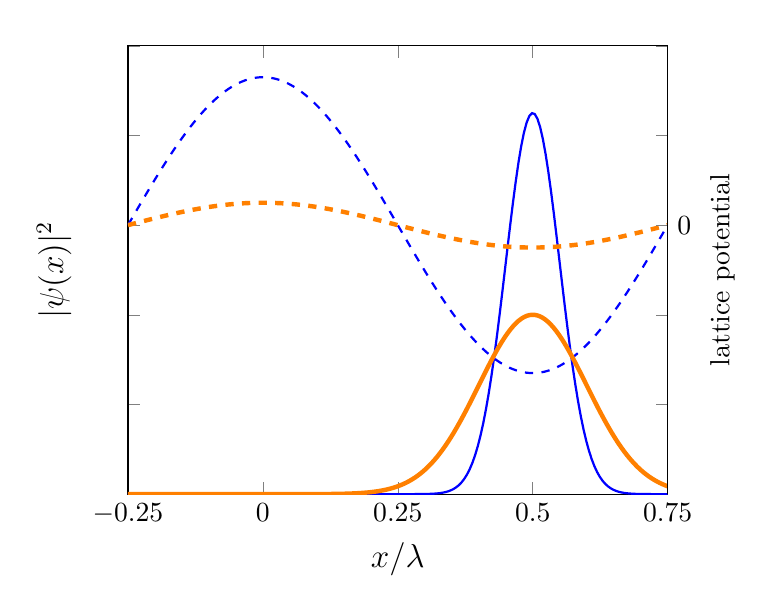
\begin{tikzpicture}
\begin{axis}[
    %title={Temperature dependence of CuSO$_4\cdot$5H$_2$O solubility},
    ylabel={$|\psi(x)|^2$},
    xlabel={$x / \lambda$},
    xmin=-.25, xmax=.75,
    ymin=0, ymax=10,
    %xtick={5},
    xtick={-0.25, 0, 0.25, 0.5, 0.75},
    %xticklabels={$\eta_\text{crit}$},
    %yticklabels={0, 0.2, 0.4, 0.6, 0.8, 1},
    yticklabel style=white,
    label style={font=\large},
    legend style={font=\small},
    legend pos=north east,
    ymajorgrids=false,
    grid style=dashed,
]
\addplot [
	restrict y to domain=0:10,
    domain=-.25:.75, 
    samples=200, 
    color=blue,
    thick,
]
{8.5 * exp(-200 *(-0.5 + x)^2)};
\addplot [
	restrict y to domain=0:10,
    domain=-.25:.75, 
    samples=200, 
    color=blue,
    dashed,
    thick,
]
{3.3*cos(6.28318530718*deg(x))+6};
\addplot [
	restrict y to domain=0:10,
    domain=-.25:.75, 
    samples=200, 
    color=orange,
    ultra thick,
]
{4 * exp(-50 *(-0.5 + x)^2)};
\addplot [
	restrict y to domain=0:10,
    domain=-.25:.75, 
    samples=200, 
    color=orange,
    dashed,
    ultra thick,
]
{0.5*cos(6.28318530718*deg(x))+6};
\end{axis}


\begin{axis}[
  ymin=0, ymax=10,
  xmin=0, xmax=10,
  hide x axis,
  axis y line*=right,
  ytick={6},
  yticklabels={0},
  ylabel={lattice potential},
  ylabel near ticks,
]
\end{axis}
\end{tikzpicture}
\end{document}